\chapter{Results} \label{chap:results}
In this chapter, the obtained results from the defined experiments in Section~\ref{sec:experiments} are presented. In Section~\ref{sec:exp_feas} we summarize the results for the feasibility of deep learning-based peripheral nerve segmentation.
Section~\ref{sec:exp_3dcontext} presents the performances for the different neural network architectures with variable access to \gls{3d} information.
In Section~\ref{sec:exp_pp} presents the impact of post-processing applied to the segmentation of the baseline architecture and the best performing \gls{3d} architecture, respectively.
Finally, Section~\ref{sec:exp_evaluation} features the results obtained concerning the inter-rater variability, to which we compared and evaluated our best performing method.
The detailed results of the individual experiments can be found in the Appendix~\ref{app:results}.

\section{Experiment 1: Feasibility} \label{sec:exp_feas} %=======================================================
We successfully trained the baseline architecture on the \gls{mrn} images. In order to gain insight in the importance of the two input images (T2 and \gls{ir}), we trained the baseline architecture three times: once on each image separately, and once with both images. The mean and \gls{sd} for each of the training runs are summarized in Table~\ref{tab:results_feasibility}. Figure~\ref{fig:results_boxplot_T2_IR_dice} features a boxplot for the \acrlong{dice}. Boxplots regarding the other metrics are situated in the appendix. The results show that the training on both images yields the highest scores for all metrics except the \acrlong{vs} for the volunteer cohort. Training using only the T2 image results in comparable results as when trained with both images, concerning the \gls{dice} and \gls{vs} metrics. However, training using only the T2 image resulted in a significantly higher \gls{hd95} when compared to training on both images. Based on these results, we decided to use both images for all further training. The training took approximately 3 hours on a NVIDIA Titan Xp independent of the input. Testing a single \gls{mrn} case, hence segmenting it, took less than 3 seconds.

\begin{table}[htbp]
   \centering
   \caption[Results for Feasibility]{Mean and \gls{sd} of the \acrlong{dice}, \acrlong{vs}, and \acrlong{hd95}. The baseline was trained and evaluated on T2-only, IR-only and on the combination of them (T2 and IR).}
   \begin{tabular}{l*{4}{l}}
      \toprule
      Cohort	& Image  & DICE              & VS				& HD95\\
      			&			&					&					& (mm)\\
      \midrule
      Patient   & T2 and IR & $\mathbf{0.704 \pm 0.139}$& $\mathbf{0.882 \pm 0.098}$ & $\mathbf{16.526 \pm 17.025}$ \\
                & T2        & $0.695 \pm 0.142 $& $0.879 \pm 0.111$ & $ 17.522 \pm 17.218$ \\
                & IR        & $0.384 \pm 0.197 $& $0.733 \pm 0.226$ & $ 23.124 \pm 17.229$ \\
      \midrule
      Volunteer & T2 and IR & $\mathbf{0.861 \pm 0.057 }$& $0.921 \pm 0.056$ & $\mathbf{1.644 \pm 2.321}$ \\
                & T2        & $0.840 \pm 0.078 $& $\mathbf{0.936 \pm 0.054}$ & $ 5.909 \pm 12.433$ \\
                & IR        & $0.648 \pm 0.097 $& $0.900 \pm 0.114$ & $ 11.974 \pm 16.394$ \\
      \bottomrule
   \end{tabular}
   \label{tab:results_feasibility}
\end{table}

\begin{figure}[htbp]
	\centering
	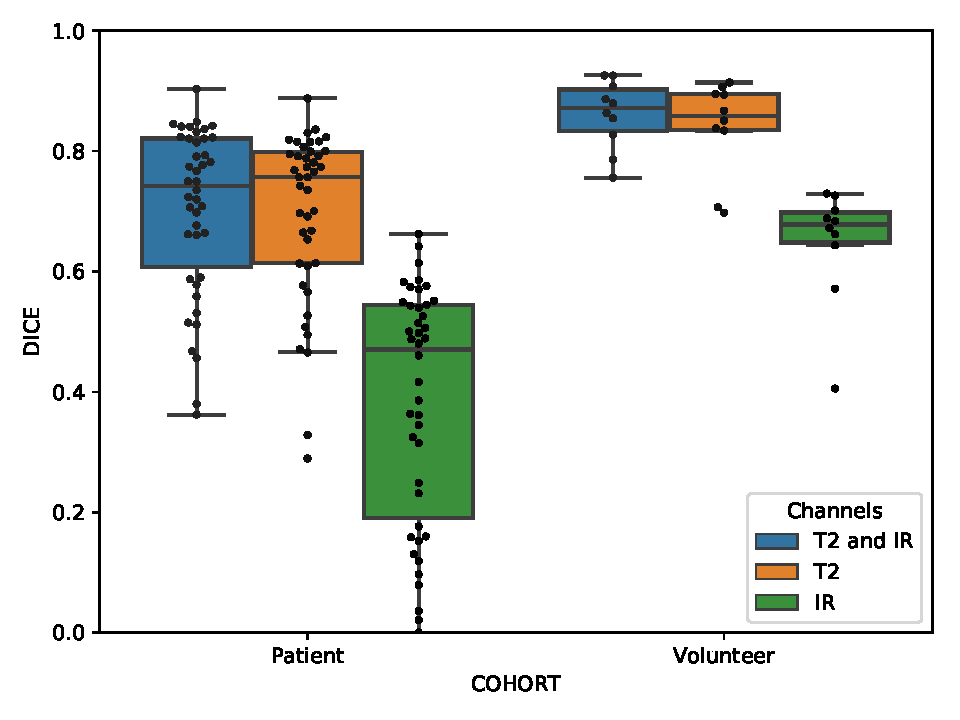
\includegraphics[width=0.8\textwidth]{boxplot_T2_IR_DICE}
    \caption[Boxplot of the \acrlong{dice} for the baseline architecture]{Boxplot of the \acrlong{dice} for the baseline architecture trained on T2 and IR, T2-only, and IR-only. Note that comparable segmentation performance is achieved by only using the T2 image. Using only the IR channel, however, results in a significantly lower performance.}
    \label{fig:results_boxplot_T2_IR_dice}
\end{figure}

\section{Experiment 2: 3-D Context} \label{sec:exp_3dcontext} % ==================================================
We successfully trained the neural networks with the proposed \gls{3d} architectures, which enables incorporating more \gls{3d} context information. The mean and \gls{sd} for the \acrlong{dice}, \acrlong{vs}, and \acrlong{hd95} are summarized in Table~\ref{tab:results_3d_context_small} together with the baseline results. A boxplot for the \acrlong{dice} is shown in Figure~\ref{fig:results_boxplot_dice}. The stack-based method achieved almost constantly better results than the baseline. The projection-based and patch-based architectures resulted in worse performance. Figure~\ref{fig:results_heatmap_dice} features a heatmap, listing the achieved \acrlong{dice}s on the patients and volunteers for all neural network architectures. The heatmap reveals that the lowest \gls{dice} values are achieved mostly on patient subjects, independent of the network architecture. Some of the outliers in the Boxplot~\ref{fig:results_boxplot_dice} are due these low \gls{dice} values. Training took 15 and 22 hours on a NVIDIA Titan Xp for the stack-wise and patch-wise neural networks, respectively. Testing a single \gls{mrn} case took less than 3 seconds. The complete results, also featuring the \acrlong{avd} and \acrlong{hd}, can be found in the appendix Table~\ref{tab:results_3d_context}.

\begin{table}[htbp]
   \centering
   \caption[Results for 3-D Context]{Mean and \gls{sd} of the \acrlong{dice}, \acrlong{vs}, and \acrlong{hd95} for different \gls{3d} context information.}
   \begin{tabular}{l*{6}{l}}
      \toprule
      Cohort	& Architecture	& DICE				& VS				& HD95\\
      			&					&					&					& (mm)\\
      \midrule
      Patient   & 2-D baseline & $0.704 \pm 0.139$ & $0.882 \pm 0.098$ & $16.526 \pm 17.025$ \\
                & Stack\_3to1  & $0.749 \pm 0.139$ & $0.896 \pm 0.123$ & $\mathbf{10.807 \pm 13.393}$ \\
                & Stack\_5to1  & $\mathbf{0.765 \pm 0.123}$ & $\mathbf{0.898 \pm 0.110}$ & $12.418 \pm 19.104$ \\
                & Stack\_5to3  & $0.717 \pm 0.135$ & $0.883 \pm 0.105$ & $19.312 \pm 22.545$ \\
                & Stack\_Proj  & $0.712 \pm 0.136$ & $0.889 \pm 0.094$ & $19.878 \pm 21.613$ \\
                & Patch & $0.682 \pm 0.128$ & $0.876 \pm 0.101$ & $24.241 \pm 20.896$ \\                
      \midrule
      Volunteer & 2-D baseline & $0.861 \pm 0.057$ & $0.921 \pm 0.056$ & $1.644  \pm 2.321 $ \\
                & Stack\_3to1  & $0.860 \pm 0.073$ & $0.925 \pm 0.043$ & $2.260  \pm 2.336 $ \\
                & Stack\_5to1  & $\mathbf{0.878 \pm 0.048}$ & $\mathbf{0.928 \pm 0.048}$ & $1.537  \pm 1.784 $ \\
                & Stack\_5to3  & $0.855 \pm 0.052$ & $0.928 \pm 0.062$ & $\mathbf{1.350  \pm 1.365} $ \\                
                & Stack\_Proj  & $0.842 \pm 0.051$ & $0.917 \pm 0.067$ & $1.642  \pm 1.549 $ \\
                & Patch & $0.806 \pm 0.068$ & $0.888 \pm 0.085$ & $7.992  \pm 13.474$ \\
      \bottomrule
   \end{tabular}
   \label{tab:results_3d_context_small}
\end{table}

\begin{figure}[htbp]
	\centering
	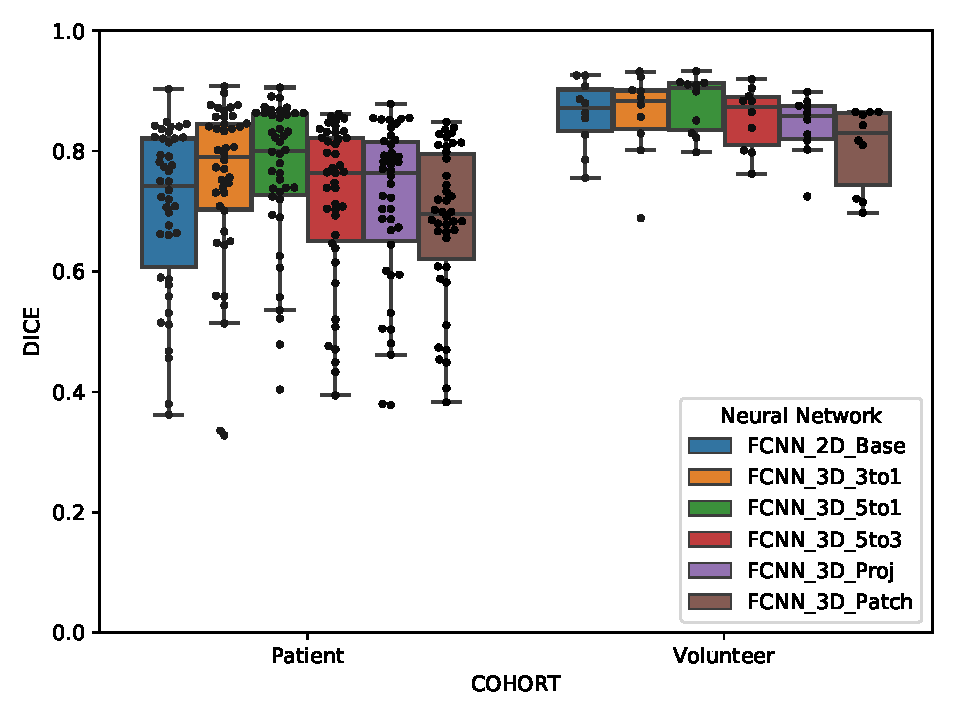
\includegraphics[width=\textwidth]{boxplot_DICE}
    \caption[Boxplot of the \acrlong{dice} for 3-D context architectures]{Boxplot of the \acrlong{dice} for the different \gls{3d} context architectures.}
    \label{fig:results_boxplot_dice}
\end{figure}

\begin{figure}[htbp]	
	\centering
	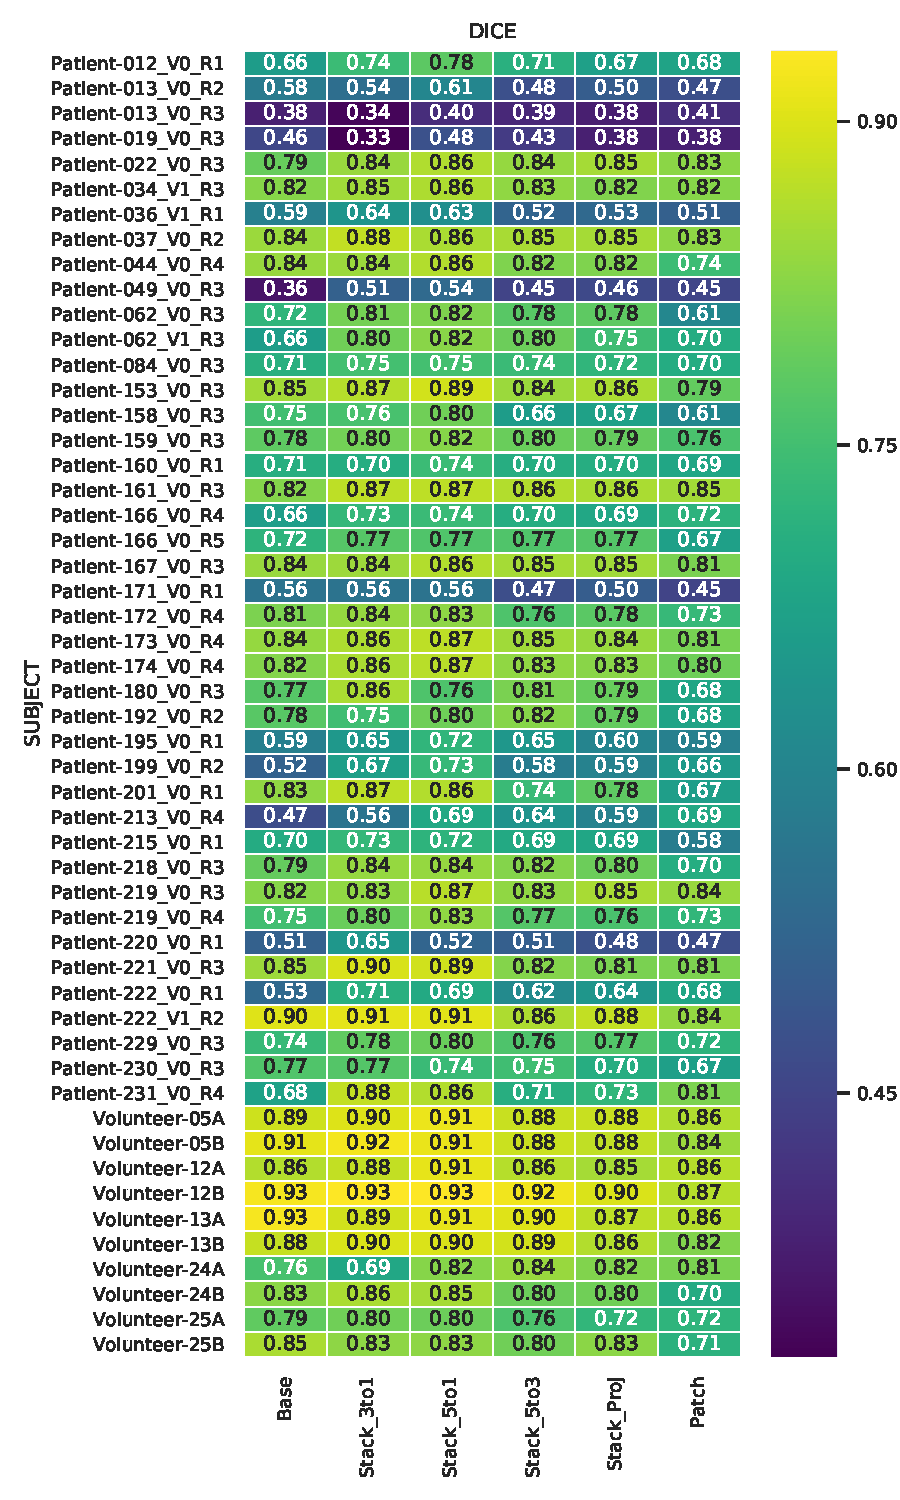
\includegraphics[width=\textwidth,height=\textheight,keepaspectratio]{heat_dice}
    \caption[Heatmap for the \acrlong{dice} for 3-D Context]{Heatmap for the achieved \acrlong{dice}s of the different neural network architectures.}
    \label{fig:results_heatmap_dice}
\end{figure}


\section{Experiment 3: Post-processing} \label{sec:exp_pp} % ====================================================
We applied the developed post-processing to the baseline and stack-based (5 to 1 slices) architecture. Post-processing was done on a desktop computer with a 6-core Intel i7 processor, and took approximately 3 minutes for keeping the $n$ largest volumes only (\textit{Volumes only}) for all 52 subjects. The number of volumes to keep was tuned for both architectures, resulting in $n = 3$ and $n = 2$ volumes for the baseline and stack-wise architecture, respectively. Joining the volumes and then keeping only the largest one (\textit{Joint volumes}) took one hour to process for all 52 subjects. Table~\ref{tab:results_pp_small} presents the obtained results with respect to the \acrlong{dice}, \acrlong{vs}, and \acrlong{hd95} (see Table~\ref{tab:results_pp} for all metrics). The overlap-based metrics were not influenced much by the post-processing but highly affected the \gls{hd95}. The boxplot in Figure~\ref{fig:pp_boxplots_hd95} shows the \acrlong{hd95} for the post-processing (see Figures~\ref{fig:pp_boxplots_vs} to \ref{fig:pp_boxplots_hd} for the other metrics). The influence of the post-processing is further shown in Figure~\ref{fig:pp_patient_219}.

\begin{table}[htbp]
   \centering
   \caption[Results for Post-processing]{Mean and \gls{sd} of the \acrlong{dice}, \acrlong{vs}, and \acrlong{hd95}. Post-processing was applied to the baseline and the stack architecture. \textit{Volumes only}: the $n$ largest volumes were kept ($n = 3$ and $n = 2$ for the Base and Stack\_5to1 architecture). \textit{Joint volumes}: connects the correctly segmented volumes first, and then keeping only the largest one.}
   \begin{tabular}{l*{7}{l}}
      \toprule
      Cohort	& Network	& Post-processing	& DICE				& VS				& HD95\\
      			&					&					&					&					& (mm)\\
      \midrule
      Patient   & Baseline 	& None & $0.705 \pm 0.137$ & $\mathbf{0.883 \pm 0.097}$ & $16.285 \pm 16.896$\\
                &                	& Volumes only  & $0.711 \pm 0.145$ & $0.867 \pm 0.125$ & $20.364 \pm 20.125$\\
                &                	& Joint volumes & $\mathbf{0.722 \pm 0.136}$ & $0.873 \pm 0.125$ & $\mathbf{11.812 \pm 12.785}$\\
      \cmidrule{2-6}
                & Stack\_5to1 	& None & $0.765 \pm 0.123$ & $0.898 \pm 0.110$ & $12.418 \pm 19.104$\\
                &                	& Volumes only  & $0.772 \pm 0.120$ & $0.899 \pm 0.119$ & $11.481 \pm 16.706$\\
                &                	& Joint volumes      & $\mathbf{0.779 \pm 0.123}$ & $\mathbf{0.905 \pm 0.117}$ & $\mathbf{6.688  \pm 10.332}$\\
      \midrule
      Volunteer & Baseline 	& None & $0.861 \pm 0.057$ & $0.921 \pm 0.056$ & $1.644  \pm 2.321 $\\
                &                	& Volumes only  & $0.862 \pm 0.057$ & $0.924 \pm 0.056$ & $2.311  \pm 4.508 $\\
                &                	& Joint volumes      & $\mathbf{0.868 \pm 0.050}$ & $\mathbf{0.929 \pm 0.056}$ & $\mathbf{1.230  \pm 1.255}$\\
      \cmidrule{2-6}
                & Stack\_5to1 	& None & $0.884 \pm 0.046$ & $0.927 \pm 0.051$ & $1.140  \pm 1.344 $\\
                &                	& Volumes only  & $0.883 \pm 0.046$ & $0.933 \pm 0.049$ & $1.357  \pm 1.454 $\\
                &                	& Joint volumes      & $\mathbf{0.894 \pm 0.042}$ & $\mathbf{0.942 \pm 0.050}$ & $\mathbf{0.655  \pm 0.355}$\\
      \bottomrule
   \end{tabular}
   \label{tab:results_pp_small}
\end{table}

\begin{figure}[htbp]
	\centering
	\subfloat[]
	{
		\label{fig:subfig:pp_boxplot_base_hd95}
		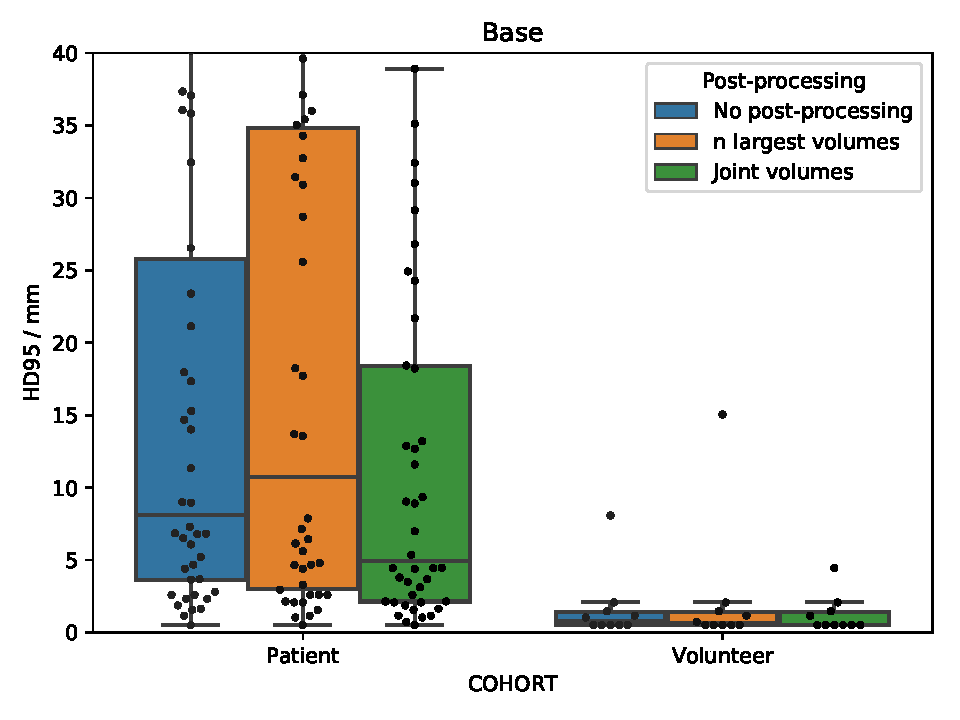
\includegraphics[width=0.7\textwidth]{pp_boxplot_base_HD95}
	}
	\hfill
	\subfloat[]
	{
		\label{fig:subfig:pp_boxplot_5to1_hd95}
		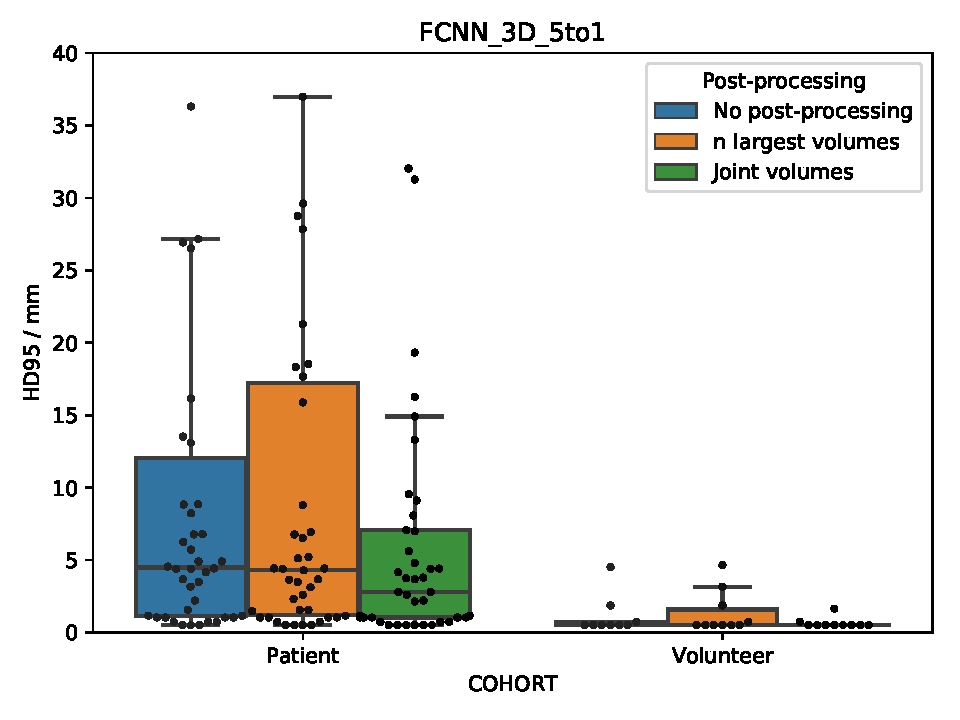
\includegraphics[width=0.7\textwidth]{pp_boxplot_5to1_HD95}
	}
	\caption[Boxplots of the \acrlong{hd95} for the post-processing]{Boxplots of the \acrlong{hd95} for the \textbf{a)} baseline and \textbf{b)} best performing stack-wise architecture with post-processing.  \textit{Volumes only}: the $n$ largest volumes were kept ($n = 3$ and $n = 2$ for the Base and Stack\_5to1 architecture). \textit{Joint volumes}: connects the correctly segmented volumes first, and then keeping only the largest one.}
	\label{fig:pp_boxplots_hd95}  
\end{figure}


\begin{figure}[htbp]
	\centering
	\subfloat[]
	{
		\label{fig:subfig:pp_base_219}
		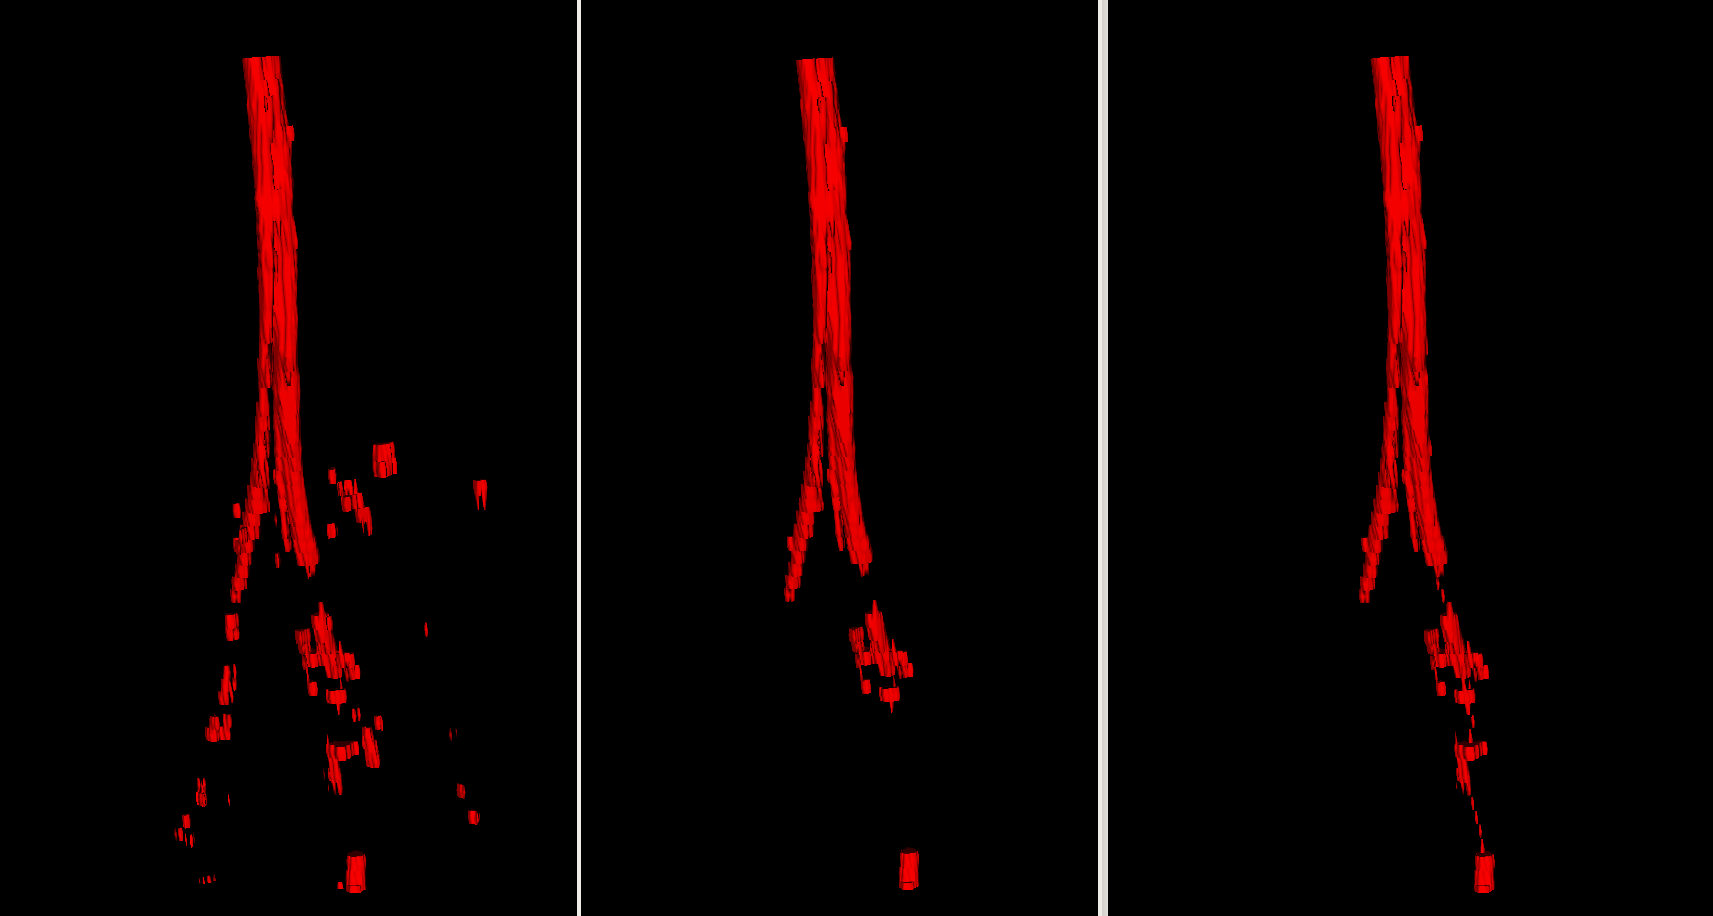
\includegraphics[width=\textwidth]{pp_base_219}
	}
	\hfill
	\subfloat[]
	{
		\label{fig:subfig:pp_5to1_219}
		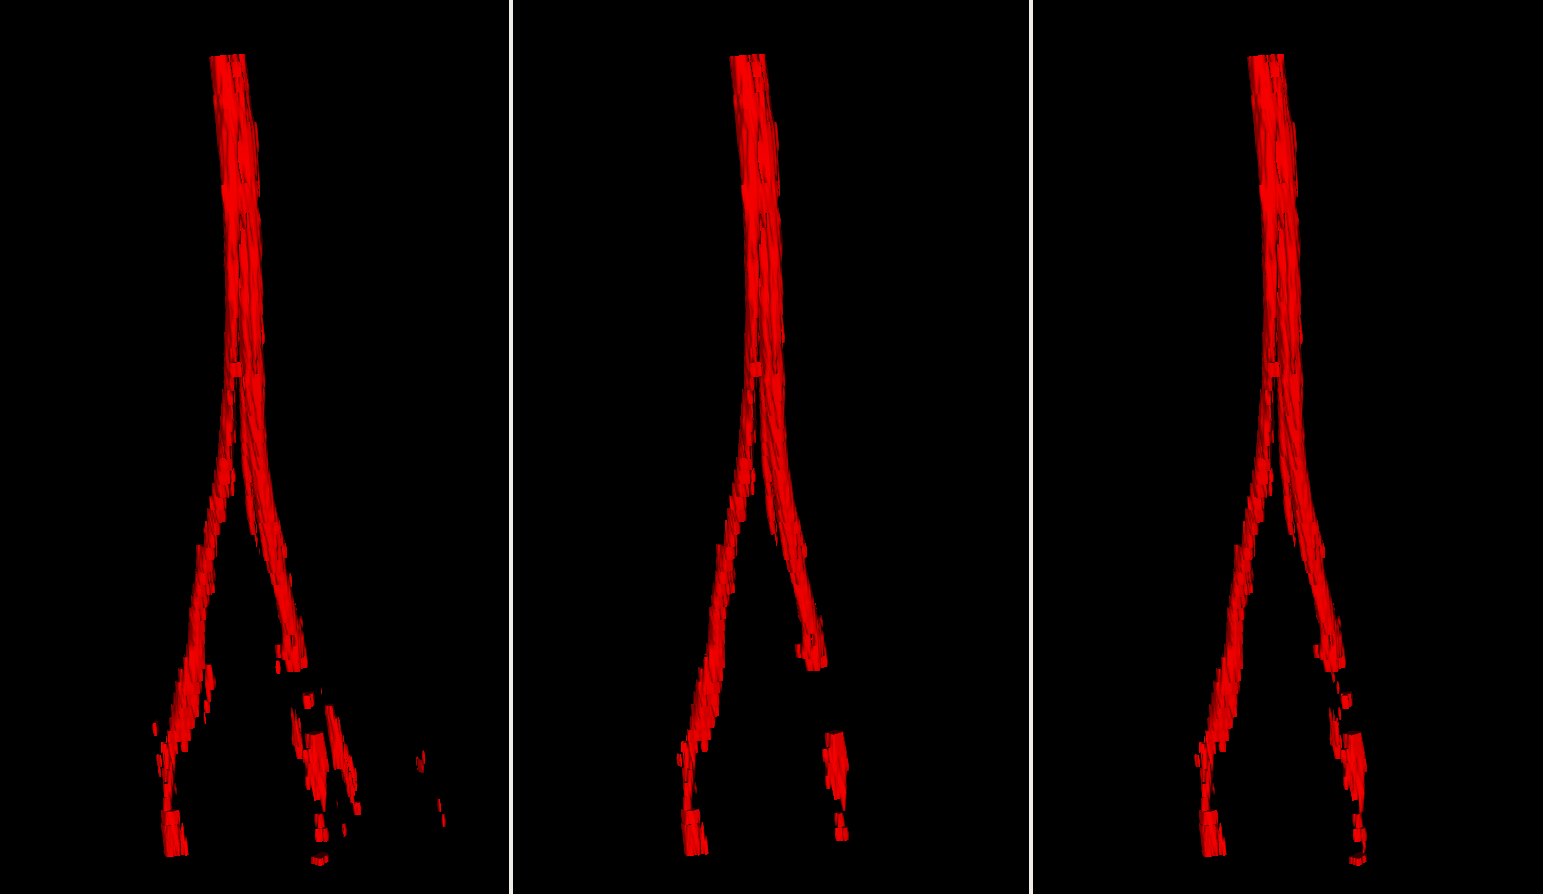
\includegraphics[width=\textwidth]{pp_5to1_219}
	}
	\caption[Segmentations Renderings]{Effect of the post-processing illustrated with \gls{3d} renderings of a segmented patient's sciatic nerve. \textbf{a)} Output segmentation of the baseline without post-processing (left), with $n$ largest volumes only (center), and with \textit{joint volumues} post-processing (right). \textbf{b)} Output segmentation of the best performing stack-wise architecture without post-processing (left), with $n$ largest volumes only (center), and with \textit{joint volumes} post-processing (right).}
	\label{fig:pp_patient_219}  
\end{figure}

\section{Comparison to Human Inter-Rater Performance} \label{sec:exp_evaluation} % ===============================================================
We compared the best performing architecture to the inter-rater agreement. The best performing architecture is the Stack-wise 5to1 with the \textit{joint volumes} post-processing (FCNN-GT; $n = 52$). The inter-rater agreement was obtained as described in Section~\ref{sec:eval_baseline} (R-R; $n = 156$).
Table~\ref{tab:res_fcnn_rater_small} summarizes the achieved \acrlong{dice}, \acrlong{vs}, and \acrlong{hd95}. Our proposed method achieves higher \gls{dice} values than the inter-rater performance. The $p$-values and the statistical significance of the comparison are gathered in the Table~\ref{tab:res_fcnn_rater_statistics}. Only for the volunteer \gls{dice} score, the difference is statistically significant. Hence, from a statistical point of view, our method is on par with the human inter-rater performance, or even surpassing it in the case of the \acrlong{dice} for the volunteer cohort.
Figure~\ref{fig:results_eval_boxplot_dice} shows the corresponding boxplot of the \acrlong{dice}. A detailed table (Table~\ref{tab:res_fcnn_rater}) and additional figures  are presented in the appendix.
In Figure~\ref{fig:res_inter_rater} the inter-rater agreement is shown as a heatmap for all the rater-to-rater and rater-to-ground-truth combinations.

\begin{table}[htbp]
   \centering
   \caption[Results for Comparison to Inter-Rater Performance]{Mean and \gls{sd} of the \acrlong{dice}, \acrlong{vs}, and \acrlong{hd95} achieved when comparing the best performing FCNN (Stack\_5to1 with full post-processing) to the inter-rater performance (R-R).}
   \begin{tabular}{l*{8}{l}}
      \toprule
      Cohort	& Comparison & DICE              & VS				& HD95\\
      			&			&					&					& (mm)\\
      \midrule
        Patient     & FCNN-GT & $0.779 \pm 0.123$ & $\mathbf{0.905 \pm 0.117}$ &                     $\mathbf{6.688  \pm 10.332}$ \\
                    & R-R     & $\mathbf{0.786 \pm 0.093}$ & $0.897 \pm 0.087$ &                     $11.245 \pm 19.008$ \\
        \midrule
        Volunteer   & FCNN-GT & $\mathbf{0.894 \pm 0.042}$ & $\mathbf{0.942 \pm 0.050}$ &                     $\mathbf{0.655  \pm 0.355} $ \\
                    & R-R     & $0.869 \pm 0.031$ & $0.937 \pm 0.043$ &                     $0.703  \pm 0.672 $ \\
      \bottomrule
   \end{tabular}
   \label{tab:res_fcnn_rater_small}
\end{table}


\begin{table}[htbp]
   \centering
   \caption[Statistics for Comparison to Inter-Rater Performance]{Statistical significance and $p$-values for the conducted unpaired Mann-Whitney U test (95 \% confidence interval) for the comparison to human inter-rater performance.}
   \begin{tabular}{l*{3}{l}}
      \toprule
        Cohort	    & Metric        & $p$       & Statistically significant\\
      			    &               &           &($p < 0.05$)          \\
      \midrule
        Patient     & \gls{dice}    & 0.60      & No\\
                    & \gls{vs}      & 0.60      & No\\
                    & \gls{avd}     & 0.31      & No\\
                    & \gls{hd95}    & 0.54      & No\\
                    & \gls{hd}      & 0.29      & No\\
        \midrule
        Volunteer   & \gls{dice}    & 0.02      & Yes\\
                    & \gls{vs}      & 0.65      & No\\
                    & \gls{avd}     & 0.70      & No\\
                    & \gls{hd95}    & 0.48      & No\\
                    & \gls{hd}      & 0.18      & No\\
      \bottomrule
   \end{tabular}
   \label{tab:res_fcnn_rater_statistics}
\end{table}

\begin{figure}[htbp]
	\centering
	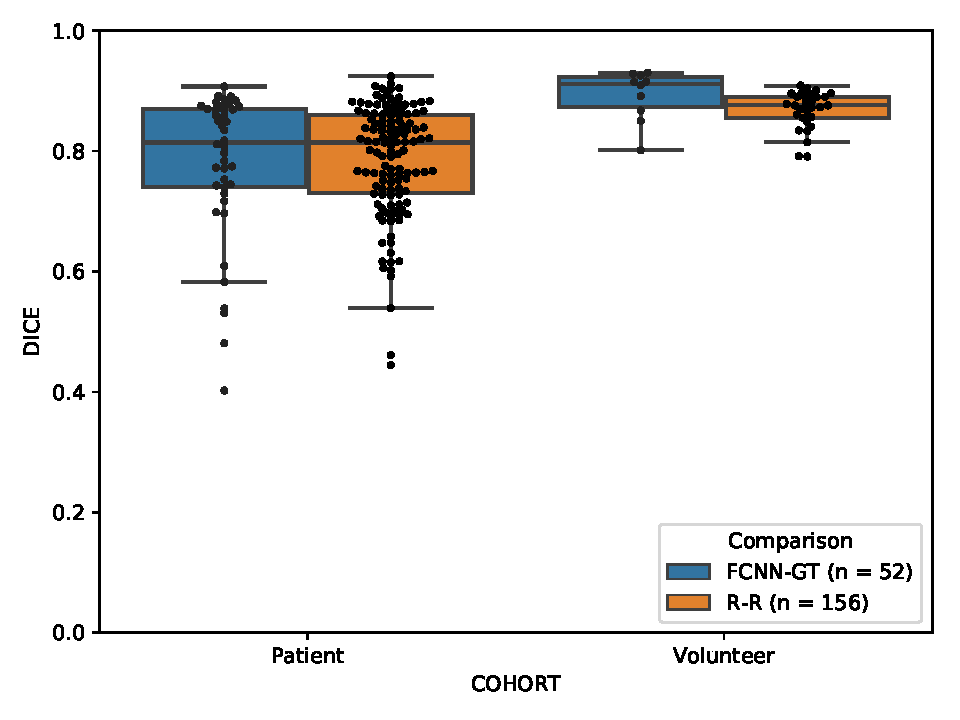
\includegraphics[width=\textwidth]{boxplot_eval_DICE}
    \caption[Boxplot of the \acrlong{dice} compared to the inter-rater performance]{Boxplot of \acrlong{dice} with the best performing architecture (FCNN-GT) and the inter-rater (R-R) performance. The best performing architecture achieves higher values for the volunteer cohort, with statistical significance. No statistically significant differences were found regarding the remaining metrics.}
    \label{fig:results_eval_boxplot_dice}
\end{figure}

\begin{figure}[htbp]	
	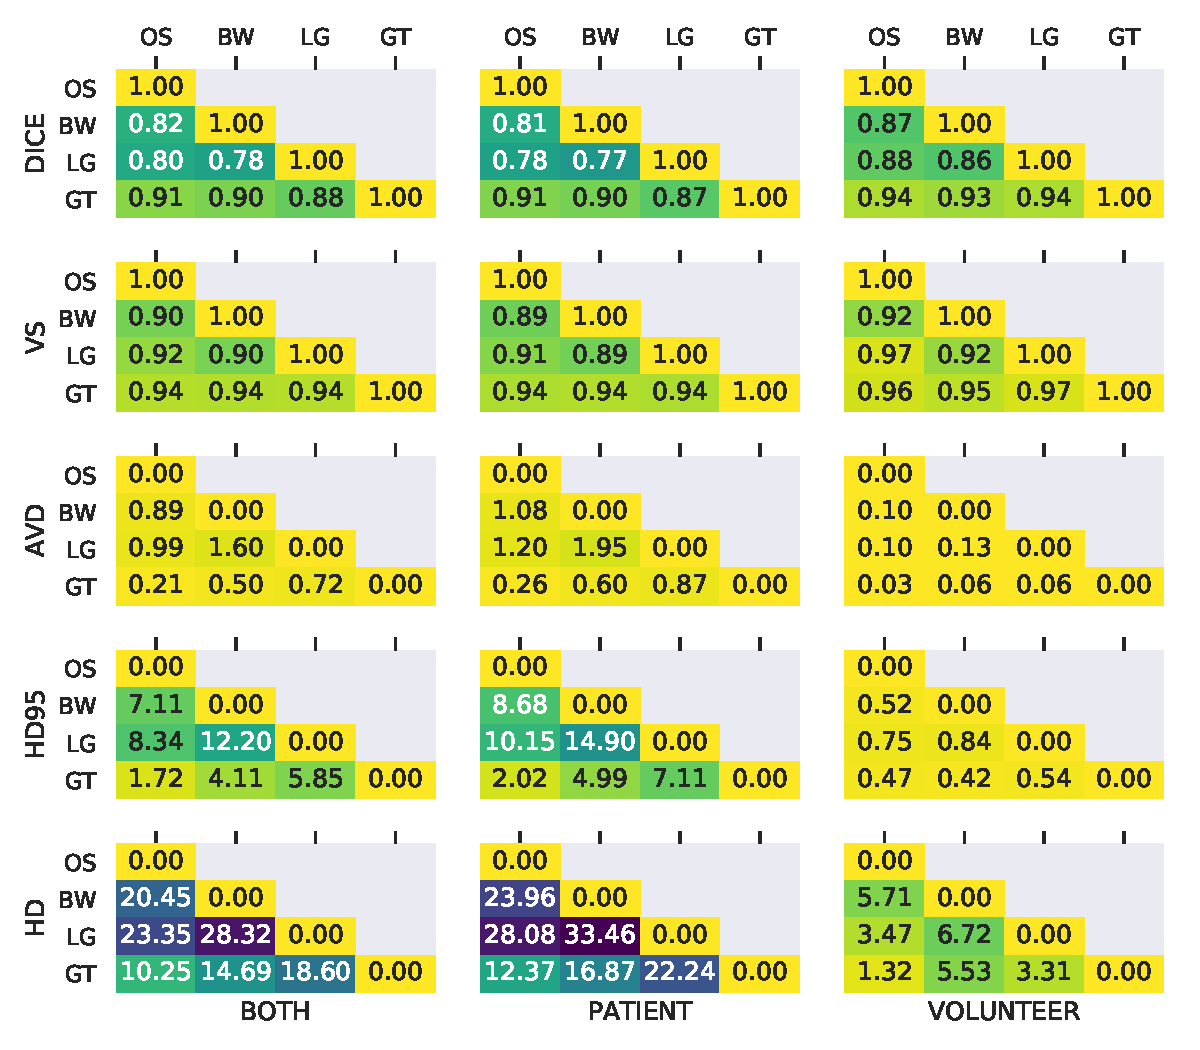
\includegraphics[width=\textwidth]{inter_rater}
    \caption[Heatmap for Inter-Rater Agreement]{Inter-rater agreement for the \acrlong{dice}, \acrlong{vs}, \acrlong{avd}, \acrlong{hd95} and \acrlong{hd} per cohort. Values close to 1.00 for \gls{dice} and \gls{vs} correspond to a high level of agreement between the raters. Conversely, low values for \gls{avd}, \gls{hd95} and \gls{hd} imply higher agreement.}
    \label{fig:res_inter_rater}
\end{figure}

\section{Time Requirements} \label{sec:res_times}
Table~\ref{tab:results_durations} contains all the different times required for the individual steps involved in the peripheral nerve segmentation. Note that the fully-automatic segmentation of one \gls{mrn} case, including registration (1 $\pm$ 0.5 minute), segmentation by the neural network (3 seconds) and \textit{joint volumes} post-processing (1 minute), takes a total of 2 $\pm$ 0.5 minutes.

\begin{table}[htbp]
   \centering
   \caption[Time Requirements]{Time requirements for the different steps involved in the peripheral nerve segmentation. All durations are given as the time required to process a single \gls{mrn} case.}
   \begin{tabular}{l*{3}{l}}
      \toprule
      Step                  & Variant               & Duration\\
      \midrule
      Training              & Base                  & 2 h   \\
                            & Stack (all)           & 15 h  \\
                            & Patch                 & 22 h  \\
      \midrule
      Registration          &                       & $1 \pm 0.5$ min \\
      \midrule
      Segmentation          &                       & 3 s \\
      Post-processing       & $n$ largest volumes   & 4 s \\
                            & Joint volumes         & 1 min \\
      \midrule
      Fully-automatic segmentation & & 2 $\pm$ 0.5 min\\
      (After training, full post-processing)\\
      \midrule
      Manual ground truth segmentation & & $19 \pm 8$ min\\
      (done by expert) \\
      \bottomrule
   \end{tabular}
   \label{tab:results_durations}
\end{table}

\endinput